\chapter[Introdução]{Introdução}

É inconcebível imaginar o mundo moderno sem software. Ele esta tão acoplado nas mais diversas áreas que seria difícil prever como o mundo seria sem o suporte e as facilidades que ele traz ao nosso dia a dia. Diante deste acoplamento tão grande e do seu enorme crescimento nos últimos anos, consequência do avanço tecnológico, se torna cada vez mais importante desenvolver software. O desenvolvimento de software pode possuir diferentes contextos de negócio, e com isso diferentes habilidades são exigidas dos desenvolvedores, já que cada contexto possui suas particularidades. Além disso, o ritmo acelerado do mundo moderno faz com que os contextos evoluam, e com isso as suas atividades e necessidades (requisitos) também evoluem. A mudança nos requisitos, a sua diversidade, e em algumas vezes a dificuldade em precisa-los, leva o desenvolvimento tradicional de software a ser lento e caro em contextos que estão sempre evoluindo \cite{lieberman2006}. Além disso, a limitação na capacidade de produção de software de uma organização pode levar à priorização das demandas, e como consequência algumas áreas de negócio podem ficar sem atendimento. Diante deste cenário, se torna cada vez mais comum aplicações de software serem desenvolvidas por desenvolvedores não profissionais, pessoas que possuem conhecimento básico em programação mas que possuem expertise em um determinado domínio. O desejo de suportar seus objetivos neste domínio através de uma solução computacional os leva a serem tanto desenvolvedores quanto usuários finais do software \cite{lieberman2006}. O Escritório do Trabalho e Estatística dos Estados Unidos fez uma previsão de que por volta de 2012, nos Estados Unidos, haveriam pouco mais de 3 milhões de programadores profissionais e mais de 55 milhões de pessoas escrevendo fórmulas e \textit{queries} em planilhas e banco de dados, para suportar seus objetivos de trabalho \cite{scaffidi2005}. Um relatório divulgado pelo \textit{Gartner} em Julho de 2011, indicou que desenvolvedores não profissionais iriam construir ao menos 25 \% das novas aplicações de negócio em 2014 \cite{paterno2013}. Diante deste cenário, um modelo de desenvolvimento de software centrado nesses usuários finais que desenvolvem cada vez mais vem ganhando força. O \textit{End User Development} - EUD tem como objetivo oferecer meios para que os usuários finais, que não são especialistas em programação, possam desenvolver aplicações de software. O EUD pode ajudar a aumentar a capacidade produtiva do departamento de TI de uma organização, bem como reduzir custos com o desenvolvimento de aplicações de negócio.

O serviço público brasileiro, por ter natureza administrativa, apresenta grande demanda por desenvolvimento de software. Porém, a limitada capacidade produtiva da área de TI e o excesso de burocracia para o aumento da mesma, que é feita através de concursos ou de contratos terceirizados, acaba contribuindo para que as demandas das áreas de negócio consideradas menos prioritárias sejam deixadas de lado \cite{artigoTcuGovTI}. O uso de planilhas e o desenvolvimento de aplicações clandestinas sem nenhuma documentação e padrão, por essas unidades de negócio, promove o desconhecimento de soluções informatizadas por parte da alta cúpula, bem como a duplicidade de esforços pelas unidades \cite{slideTCU}. Nesse sentido, alguns órgãos da administração pública federal vêm reconhecendo esses esforços feitos informalmente pelas áreas de negócio, e começaram a adotar o modelo EUD, com algumas adaptações, para tentar contornar os problemas relatados. Os órgãos vem chamando esse modelo de modelo de desenvolvimento descentralizado, uma espécie de EUD onde o usuário final não é necessariamente quem desenvolve as aplicações. Geralmente estagiários da área de TI são contratados, para que eles possam ser alocados nas unidades de negócio do órgão, de forma que eles desenvolvam as aplicações junto à área de negócio, com a consultoria técnica da área de TI \cite{slideTCU}. Uma iniciativa bem sucedida de desenvolvimento descentralizado já foi implantada em um órgão da administração pública federal, com um relato de alta satisfação dos usuários. Apesar disso, ainda existem algumas dificuldades no desenvolvimento por parte dos estagiários, que não possuem um guia/processo que os oriente durante todo o ciclo de desenvolvimento. Por serem estagiários, muitos acabam seguindo a forma de desenvolvimento e os padrões que acreditam serem os melhores, o que acaba colocando em dúvida a qualidade das aplicações desenvolvidas. 

Dentro deste contexto, o objetivo geral deste trabalho é desenvolver uma solução de apoio ao desenvolvimento EUD (descentralizado) para um orgão público federal, agregando recursos que promovam a qualidade dos sistemas desenvolvidos, a partir de princípios e conceitos de engenharia de software.

Considerando o objetivo geral, foram definidos os seguintes objetivos específicos:

\begin{enumerate}
\item Entender o contexto do EUD no orgão público alvo.
\item Diagnosticar os problemas no desenvolvimento de aplicações baseado em EUD.
\item Selecionar as práticas da engenharia de software que sejam adequadas à solução dos problemas encontrados e ao contexto.
\item Elaborar o modelo conceitual da solução de apoio.
\item Construir a solução de apoio.
\item Selecionar um projeto para a aplicação da solução.
\item Aplicar a solução de apoio no projeto selecionado.
\item Relatar os resultados obtidos.
\end{enumerate}


\begin{comment}
Apesar disso, existem ainda algumas dificuldades no desenvolvimento por parte dos estagiários desenvolvedores, como a falta de padronização e o que demonstra a necessidade de a elaboração de um processo embasado por princípios em conceitos da engenharia de software, ao mesmo tempo que não seja custoso aos desenvolvedores, já que iria contra a flexibilidade que preconiza o modelo EUD. 

\citeonline{lieberman2006} relatou que um dos objetivos da interação humano-computador, além de desenvolver sistemas que são fáceis de usar, seria desenvolver sistemas que são fáceis de desenvolver.
\end{comment}

\chapter[Referencial Teórico]{Referencial Teórico}

Esta seção apresenta o referencial que embasa este trabalho. O referencial teórico é o meio em que o autor do trabalho demonstra o seu conhecimento sobre uma determinada área de estudo (teorias, vocabulários, variáveis chave, fenômenos, métodos e história) \cite{randolph2009}.


\section{\textit{End User Development}}

\textit{End User Development} (Desenvolvimento por usuário final) é um modelo de desenvolvimento de software onde o usuário final é o principal responsável pela construção do software. \citeonline{lieberman2006} define o \textit{End User Development} (EUD) como um conjunto de métodos, técnicas e ferramentas que permite aos usuários de sistemas de software, que agem como desenvolvedores de software não profissionais, em algum ponto, criar, modificar ou estender um artefato de software. Dentre as motivações para este modelo de desenvolvimento, destacam-se a diversidade e a mutabilidade dos requisitos, bem como a dificuldade em defini-los em contextos que evoluam com uma alta frequência, o que pode levar o desenvolvimento tradicional a consumir muito tempo e atingir um alto custo \cite{lieberman2006}. Além disso, uma organização que possui uma demanda por informatização dos seus processos de trabalho, por parte das suas diferentes áreas de negócio, superior a capacidade produtiva da área de TI, pode não conseguir atender certas áreas por conta das priorizações das demandas \cite{artigoTcuGovTI}. O EUD acelera as respostas às mudanças e contorna o problema de precisão dos requisitos, porque os usuários finais geralmente são especialistas no domínio em que estão inseridos, ou seja, são os detentores dos requisitos da solução computacional \cite{fischer2004}. O fato de cada usuário final ser um potencial desenvolvedor também contribui para um aumento da capacidade produtiva da TI.

Para que o desenvolvimento seguindo este modelo possa ocorrer é necessário que existam meios para que o usuário final possa desenvolver e adaptar o software, e para tanto a tecnologia envolvida deve diminuir o esforço cognitivo necessário para a construção do software, através da aproximação conceitual entre as ações do mundo real e as do mundo da programação \cite{fischer2004}. Os usuários finais geralmente não possuem habilidades de um profissional da área de software, e também não estão interessados em construir sistemas no mesmo nível que esses profissionais, por isso é necessário que a tecnologia usada no desenvolvimento alinhe a complexidade relacionada a esta atividade com as habilidades do usuário final. A motivação dos usuários finais é algo essencial para o favorecimento deste modelo, e fatores como o empoderamento, a velocidade de desenvolvimento, a flexibilidade e o controle influenciam diretamente na motivação desses usuários.

O principal objetivo do EUD é oferecer meios para que os usuários finais consigam desenvolver e adaptar software \cite{lieberman2006}. Desta maneira, as aplicações preparadas para o EUD devem ser, principalmente, flexíveis, fáceis de se entender, de se usar, e de se ensinar \cite{lieberman2006}. A preocupação com a tecnologia usada neste modelo de desenvolvimento, mais especificamente na parte das linguagens de programação e aplicações de desenvolvimento, é a relação escopo de aplicação versus esforço de aprendizagem. A figura 1 ilustra a relação do escopo de aplicação e do custo de aprendizagem, para diferentes linguagens de programação e aplicações. Linguagens de programação mais tradicionais como C++ e JAVA oferecem a possibilidade de construção de software de uma grande variedade de domínios, porém a um alto custo associado ao esforço de aprendizagem. Outras linguagens possuem um menor esforço de aprendizagem, ao custo de uma limitação no escopo de aplicação. As linguagens ou aplicações de desenvolvimento ideais para o EUD são as que possuem um alto escopo de aplicação e um baixo esforço de aprendizagem \cite{fischer2004}. As que existem atualmente só utilizam uma pequena parte do potencial do EUD, com algumas falhas \cite{paterno2013}.

\begin{figure}[h]
	\centering
	\label{fig01}
		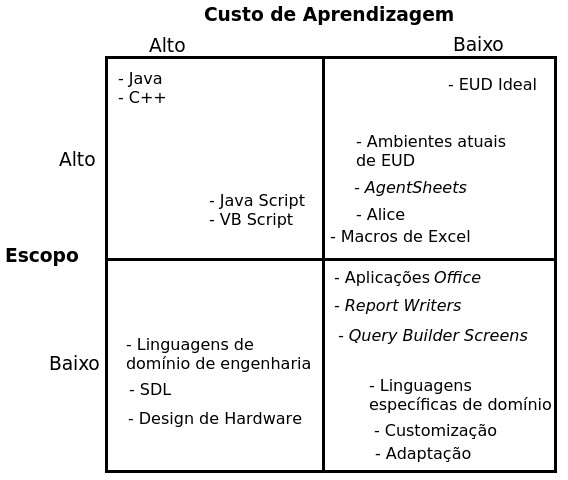
\includegraphics[scale=0.8]{figuras/trade_off_eud_editado}
	\caption{Relação escopo de aplicação e custo de aprendizagem}
\end{figure}
\pagebreak

\citeonline{lieberman2006} classifica as atividades do usuário final em dois tipos:

\begin{enumerate}
\item \textbf{Parametrização ou Customização:} São atividades que permitem o usuário escolher comportamentos, apresentações e mecanismos  alternativos, que já existem dentro de uma aplicação.

\item \textbf{Criação e modificação de programas:} São atividades que implicam na criação ou modificação de artefatos de software. Macros e linguagens de \textit{script} são exemplos deste tipo de atividade.
\end{enumerate}


\chapter[Metodologia]{Metodologia}

\textit{\{Acrescentar aqui uma breve descrição da metodologia escolhida.\}}

As pesquisas científicas, de acordo com \citeonline{gil2002}, são classificadas em três grandes grupos, segundo os seus objetivos gerais: exploratórias, descritivas e explicativas.

Destes três grupos, a pesquisa exploratória, em particular, tem como objetivo proporcionar o aprimoramento e/ou a descoberta de idéias, a respeito de um determinado problema. Proporcionando uma maior familiaridade com o problema, esse tipo de pesquisa o torna mais explícito e contribui para a construção de hipóteses em cima do mesmo. Por conta disso, a pesquisa exploratória possui um caráter flexível em seu planejamento, e geralmente assume as formas de pesquisa bibliográfica ou estudo de caso \cite{gil2002}.

O estudo de caso consiste no estudo profundo e exaustivo de um ou mais objetos, de forma a obter conhecimento amplo e detalhado sobre o mesmo. Segundo \citeonline{yin2001estudo} o estudo de caso é a abordagem mais adequada para a investigação de um fenômeno em seu contexto real, onde os limites entre este fenômeno e o seu contexto não são claramente percebidos. Os propósitos do estudo de caso são \cite{gil2002}:

\begin{itemize}
\item Explorar situações de contextos reais onde os limites não estão claramente definidos.
\item Preservar o caráter unitário do objeto.
\item Descrever a situação do contexto do qual esta sendo feita a investigação.
\item Desenvolver teorias e formular hipóteses.
\item Determinar as causas de um determinado fenômeno onde a complexidade não permite o uso de levantamentos e experimentos.
\end{itemize}

Existem diversos métodos de coleta de dados para suportar os propósitos de um estudo de caso, e um dos métodos comumente usados nos estudos de caso na engenharia de software é a entrevista \cite{caseStudySE}. Quase todos os estudos de caso envolvem algum tipo de entrevista, seja para a finalidade primária de coleta dados, seja para uma validação de outros tipos de dados \cite{caseStudySE}. A entrevista é caracterizada como um método de coleta de dados onde o pesquisador está em contato direto com os entrevistados e como um método de coleta de dados em tempo real \cite{caseStudySE}. O diálogo entre o entrevistador e o entrevistado é guiado por um conjunto de perguntas, que podem ser classificadas como abertas ou fechadas \cite{caseStudySE}. As perguntas abertas permitem uma maior gama de respostas e relatos de problemas, por parte do entrevistado. Já as perguntas fechadas oferecem alternativas mais limitadas, se comparadas as perguntas abertas. Ambos os tipos de perguntas são baseadas nos tópicos de interesse relacionados ao estudo de caso. 

Segundo \cite{caseStudySE}, a entrevista pode ser classificada em três categorias diferentes:
\begin{enumerate}
\item \textbf{Não-estruturada}: As perguntas são formuladas de forma aberta e de acordo com os interesses do pesquisador. A conversa durante a entrevista irá se desenvolver de acordo com os interesses do entrevistado e do entrevistador.
\item \textbf{Semiestruturada}: As questões planejadas não são necessariamente perguntadas na ordem em que estão listadas, tendo o desenvolvimento da conversa influência direta na ordem em que as perguntas são feitas ao entrevistado. Além disso, esse tipo de pesquisa permite o improvisamento e a exploração de problemas levantados durante a conversa. É comum em estudos de caso em engenharia de software.
\item \textbf{Completamente estruturada}: Todas as perguntas são detalhadamente planejadas de antemão e são feitas exatamente na ordem em que estão listadas. Esse tipo de entrevista se assemelha a \textit{surveys} baseados em questionários, pois se trata de perguntas fechadas.
\end{enumerate}
	
Uma vez que os dados são coletados, o foco se volta para a análise e interpretação dos mesmos. O objetivo desta etapa é derivar conclusões dos dados, buscando a compreensão e a formação de padrões em cima dos mesmos, através de uma cadeia de evidência. Uma cadeia de evidência significa que o leitor pode chegar aos mesmos resultados e conclusões em cima dos dados coletados \cite{caseStudySE}. A análise e interpretação dos dados pode ser dividida nos seguintes procedimentos \cite{caseStudySE}:

\begin{enumerate}
\item Os dados são codificados de forma que a cada pedaço do texto, que pode ser uma linha ou um parágrafo por exemplo, é atribuído um código que pode representar um certo tema, uma área, uma construção e assim por diante. Observa-se que um pedaço de texto pode possuir mais de um código e um código pode estar associado a mais de um pedaço de texto.
\item Identificar um conjunto de hipóteses em cima dos dados codificados.
\item Formar um conjunto de generalizações/conclusões.
\item Relatar os resultados.
\end{enumerate}

\section{Metodologia Adotada}

A metodologia adotada para este trabalho foi o estudo de caso, devido a necessidade de realizar um diagnóstico da situação atual para a construção da solução de apoio, e o método utilizado no estudo de caso foi a entrevista, por ser um método bastante comum neste tipo de metodologia e permitir um contato direto com os entrevistados. 

A entrevista elaborada pode ser classificada como semiestruturada, já que as perguntas foram feitas na ordem em que foram planejadas e improvisos foram feitos durante a condução da entrevista. No planejamento da entrevista, algumas categorias de perguntas relacionadas ao ciclo de vida do software e ao contexto do desenvolvedor foram elaboradas, de forma a auxiliar na formulação das perguntas. As categorias elaboradas foram:

\begin{itemize}
\item \textbf{Descrição do desenvolvedor} 

- Objetivo: Obter informações sobre o perfil dos desenvolvedores.
\item \textbf{Papel do desenvolvedor}

- Objetivo: Obter informações sobre o papel do desenvolvedor no órgão.
\item \textbf{Efetividade do curso}

- Objetivo: Obter informações sobre a preparação dos novos desenvolvedores.
\item \textbf{Requisitos}

- Objetivo 1: Obter informações sobre como se dá o levantamento de requisitos nos departamentos da instituição.

- Objetivo 2: Obter informações de como é armazenado e gerenciado os requisitos do sistema a ser desenvolvido.

- Objetivo 3: Obter informações de como é englobado as mudanças de requisitos ao sistema.
\item \textbf{\textit{Design}}

- Objetivo: Obter informações sobre como é realizado a modelagem (arquitetura) do sistema.
\item \textbf{Codificação}

- Objetivo 1: Obter informações sobre a depuração de erros do sistema.

- Objetivo 2: Obter informações sobre estilos de codificação.

- Objetivo 3: Obter informações sobre o ambiente de codificação.

\item \textbf{Teste}

- Objetivo: Obter informações sobre a realização dos testes, bem como a forma de realizá-los.
\item \textbf{Implantação}

- Objetivo: Obter informações sobre a migração, para a produção, do sistema.
\end{itemize}

A partir das categorias definidas, foram derivadas as perguntas relacionadas a cada categoria, de forma que estivessem alinhadas ao contexto do desenvolvimento descentralizado. A entrevista elaborada pode ser vista no Anexo A.

Uma vez que a entrevista foi elaborada, o foco voltou-se ao planejamento da análise dos dados da mesma. Para isso, a análise planejada consistiu dos seguintes passos:

\begin{enumerate}
\item Atribuir um código, previamente estabelecido, a uma unidade de resposta, que pode ser uma frase ou um conjunto de frases que tratem de um mesmo assunto.
\item Agrupar as unidades de resposta de acordo com as categorias de código que receberam.
\item Dentro de uma categoria de código, agrupar as unidades de respostas semelhantes.
\item Elaborar ações para as unidades de respostas agrupadas dentro das categorias de códigos.
\end{enumerate}

Os códigos elaborados foram derivados dos objetivos de cada categoria de perguntas do ciclo de vida relacionado ao contexto do desenvolvedor. A Tabela \ref{tab01} ilustra os códigos derivados de cada objetivo definido.

\begin{table}[h]
	\centering
	\begin{tabular}{|m{4.8cm} | m{4.8cm} | m{4.8cm}|}
		\hline
		\textbf{Categoria} & \textbf{Objetivo} & 
		\textbf{Código Derivado} \\ \hline
		Descrição do desenvolvedor & Obter informações sobre o perfil dos desenvolvedores & 
		Perfil do Desenvolvedor \\ \hline
		Papel do desenvolvedor & Obter informações sobre o papel do desenvolvedor no órgão & 
		Papel do Desenvolvedor \\ \hline 
		Efetividade do curso & Obter informações sobre a preparação dos novos desenvolvedores & 
		Preparação \\ \hline 
		Requisitos & Obter informações sobre como se dá o levantamento de requisitos nos departamentos da instituição & Elicitação de Requisitos \\ \cline{2-3}
		& Obter informações de como é armazenado e gerenciado os requisitos do sistema a ser desenvolvido &
		 Gerenciamento de Requisitos \\ \cline{2-2}
		& Obter informações de como é englobado as mudanças de requisitos ao sistema & \\ \hline
		\textit{Design} & Obter informações sobre como é realizado a modelagem (arquitetura) do sistema &
		Modelagem do sistema \\ \hline
		Codificação & Obter informações sobre a depuração de erros do sistema & Depuração \\ \cline{2-3}
		& Obter informações sobre estilos de codificação & Estilos de codificação \\ \cline{2-3}
		& Obter informações sobre o ambiente de codificação & Ambiente de codificação \\ \hline
		Teste & Obter informações sobre a realização dos testes, bem como a forma de realiza-los &
		Teste \\ \hline
		Implantação & Obter informações sobre a migração, para a produção, do sistema & Implantação \\
		\hline
	\end{tabular}

	\caption{Códigos elaborados para a análise dos resultados}
	\label{tab01}
\end{table}

\chapter[Resultados]{Resultados}

\begin{itemize}
\item C1 - Papel claro dentro da instituição
\item C2 - Papel que exige grande responsabilidade dentro da instituição
\item C3 - Papel definido com falta de metas
\item C4 - Contribuição relevante para a instituição
\item C5 - Curso da somente uma introdução
\item C6 - O curso poderia ser melhorado
\item C7 - Algumas aplicações com baixa qualidade
\item C8 - Construção de um catálogo de informações APEX
\item C9 - Treinamento em boas práticas APEX
\item C10 - Esclarecer como funcionada o sistema de desenvolvimento descentralizado
\item C11 - Os requisitos são levantados através de reuniões
\item C12 - Requisitos óbvios não anotados durante as reuniões são esquecidos
\item C13 - Uso de prototipagem para levantar/validar requisitos
\item C14 - Registro de requisitos em papel
\item C15 - Registro de requisitos em sistemas distintos em rede
\item C16 - Registro de requisitos inexistente
\item C17 - Reuniões constantes
\item C18 - Não atualiza o modelo de dados
\item C19 - Não valida o modelo de dados com área técnica
\item C20 - Possibilidade de gerar o modelo de dados a partir das tabelas
\item C21 - Negligência ao modelo de dados
\item C22 - Valida o modelo de dados com área técnica.
\item C23 - Elabora o modelo de dados utilizando ferramentas CASE
\item C28 - Falta do uso de um padrão de boas práticas comprometeu a qualidade da aplicação
\item C29 - Escrita legível de código
\item C30 - Mais da metade da aplicação é composta de algum código
\item C31 - Preferência pelo uso de componentes padrões do APEX
\item C32 - Aplicação bem desenvolvida
\item C33 - Boas práticas: Nomes significativos, uso de comentários, identação, padrão de nomenclatura, desenvolver pensando nas manutenções futuras, sempre usar filtros nas consultas SQL, legibilidade do código e uso de componentes padrões do APEX sempre que possível.
\item C34 - Falta de um padrão de boas práticas
\item C35 - Reutilização de código
\item C36 - Uso de editores externos
\item C37 - Uso do editor do APEX
\item C38 - Uso de testes funcionais
\item C39 - Uso de teste de comandos SQL
\item C40 - Teste de execução de páginas
\item C41 - Sem armazenamento dos resultados de teste
\item C42 - Não há elaboração de casos de teste
\item C43 - Favorável a proposta de automação de testes funcionais
\item C44 - Costuma verificar se os apelidos não estão duplicados
\item C45 - Não migra as definições de objetos
\item C46 - Navegação feita, antes de migrar, somente nas páginas que alterou
\item C47 - Navegação feita, antes de migrar, em todas as páginas da aplicação
\item C48 - Verifica a criação das tabelas no espaço de produção
\item C49 - Faz a migração da definição dos objetos de dados
\item C50 - Faz a homologação das aplicações antes de disponibilizar definitivamente na produção
\item C51 - Seria interessante o uso de uma ferramenta que mostrasse as diferença dos objetos no desenvolvimento a na produção\newline\newline
\end{itemize} Respostas que geraram as chaves acima:\newline

\begin{table}[h]
	\centering
	\begin{tabular}{|m{4.8cm} | m{4.8cm} |}
		\hline
		\textbf{Etapa} & \textbf{Pergunta - Chave Associada} \\ \hline
		Papel do desenvolvedor & Pergunta 1 - C1 \\ \cline{2-2}
		& Pergunta 2 - C4 \\ \cline{2-2}
		\hline
		Efetividade do curso & Pergunta 1 - C5 \\ \cline{2-2}
		& Pergunta 2 - C6 \\ \cline{2-2}
		& Pergunta 3 - C7 e C28 \\ \cline{2-2}
		\hline
		Requisitos & Pergunta 1 - C11 \\ \cline{2-2}
		 & Pergunta 2 - C11 \\ \cline{2-2}
		& Pergunta 3 - C14 e C15 \\ \cline{2-2}
		& Pergunta 4 - C17 \\ \cline{2-2}
		 \hline
		\textit{Design} & Pergunta 1 - C18 \\ \cline{2-2}
		& Pergunta 2 - C19 \\ \cline{2-2}
		 \hline
		Codificação & Pergunta 1 - C32 \\ \cline{2-2}
		& Pergunta 2 - C29 \\ \cline{2-2}
		& Pergunta 3 - C33 \\ \cline{2-2}
		& Pergunta 4 - C36 \\ \cline{2-2}
		& Pergunta 5 - C24 \\ \cline{2-2}
		& Pergunta 6 - C27 \\ \cline{2-2}
		& Pergunta 7 - C33 \\ \cline{2-2} \hline
		Boas práticas e padrões & Pergunta 1 - C33 e C35 \\ \cline{2-2}
		& Pergunta 2 - C33 \\ \cline{2-2}
		\hline
		Teste & Pergunta 1 - C38 \\ \cline{2-2}
		& Pergunta 2 - C40 \\ \cline{2-2}
		& Pergunta 3 - C40 e C41 \\ \cline{2-2}
		& Pergunta 4 - C42 \\ \cline{2-2}
		& Pergunta 5 - C43 \\ \cline{2-2}
		\hline
		Implantação & Pergunta 1 - C45 \\ \cline{2-2}
		& Pergunta 2 - C44 \\ \cline{2-2}
		& Pergunta 3 - C46 \\ \cline{2-2}
		& Pergunta 4 - C48 \\ \cline{2-2}
		\hline
		Observações & Observação 1 - C51 \\ \cline{2-2} 
		& Observação 2 - C12 \\ \cline{2-2} 
		& Observação 3 - C20 \\
		\hline
	\end{tabular}

	\caption{Chaves geradas pelas repostas do Desenvolvedor 1}
	\label{tab02}
\end{table}

\begin{table}[h]
	\centering
	\begin{tabular}{|m{4.8cm} | m{4.8cm} |}
		\hline
		\textbf{Etapa} & \textbf{Pergunta - Chave Associada} \\ \hline
		Papel do desenvolvedor & Pergunta 1 - C3 \\ \cline{2-2}
		& Pergunta 2 - C4 \\ \cline{2-2}
		\hline
		Efetividade do curso & Pergunta 1 - C5 \\ \cline{2-2}
		& Pergunta 2 - C6 \\ \cline{2-2}
		& Pergunta 3 - C7 e C32 \\ \cline{2-2}
		\hline
		Requisitos & Pergunta 1 - C11 \\ \cline{2-2}
		 & Pergunta 2 - C11 \\ \cline{2-2}
		& Pergunta 3 - C14 \\ \cline{2-2}
		& Pergunta 4 - C17 \\ \cline{2-2}
		\hline
		\textit{Design} & Pergunta 1 - C18 \\ \cline{2-2}
		& Pergunta 2 - C19 \\ \cline{2-2}
		\hline
		Codificação & Pergunta 1 - C30 \\ \cline{2-2}
		& Pergunta 2 - C29 \\ \cline{2-2}
		& Pergunta 3 - C33 \\ \cline{2-2}
		& Pergunta 4 - C36 \\ \cline{2-2}
		& Pergunta 5 - C24 \\ \cline{2-2}
		& Pergunta 6 - C27 \\ \cline{2-2}
		& Pergunta 7 - C33 \\ \cline{2-2} \hline
		Boas práticas e padrões & Pergunta 1 - C33 \\ \cline{2-2}
		& Pergunta 2 - C8\\ \cline{2-2}
		\hline
		Teste & Pergunta 1 - C38 e C50 \\ \cline{2-2}
		& Pergunta 2 - C40 \\ \cline{2-2}
		& Pergunta 3 - C41 \\ \cline{2-2}
		& Pergunta 4 - C42 \\ \cline{2-2}
		& Pergunta 5 - C43 \\ \cline{2-2}
		\hline
		Implantação & Pergunta 2 - C44 \\ \cline{2-2}
		& Pergunta 3 - C40 e C46 \\ \cline{2-2}
		& Pergunta 4 - C48 \\ \cline{2-2}
		\hline
		Observações & Observação 1 - C40 \\ \cline{2-2}  
		& Observação 2 - C50 \\
		\hline
	\end{tabular}

	\caption{Chaves geradas pelas repostas do Desenvolvedor 2}
	\label{tab03}
\end{table}

\begin{table}[h]
	\centering
	\begin{tabular}{|m{4.8cm} | m{4.8cm} |}
		\hline
		\textbf{Etapa} & \textbf{Pergunta - Chave Associada} \\ \hline
		Papel do desenvolvedor & Pergunta 1 - C1 \\ \cline{2-2}
		& Pergunta 2 - C4 \\ \cline{2-2}
		\hline
		Efetividade do curso & Pergunta 1 - C5 \\ \cline{2-2}
		& Pergunta 2 - C6 \\ \cline{2-2}
		& Pergunta 3 - C28 \\ \cline{2-2}
		\hline
		Requisitos & Pergunta 1 - C11 \\ \cline{2-2}
		 & Pergunta 2 - C11 \\ \cline{2-2}
		& Pergunta 3 - C15 \\ \cline{2-2}
		& Pergunta 4 - C17 \\ \cline{2-2}
		\hline
		\textit{Design} & Pergunta 1 - C21 \\ \cline{2-2}
		& Pergunta 2 - C22 \\ \cline{2-2}
		\hline
		Codificação & Pergunta 1 - C30 \\ \cline{2-2}
		& Pergunta 2 - C33 \\ \cline{2-2}
		& Pergunta 3 - C33 \\ \cline{2-2}
		& Pergunta 4 - C36 e C37 \\ \cline{2-2}
		& Pergunta 5 - C26 \\ \cline{2-2}
		& Pergunta 6 - C27 \\ \cline{2-2}
		& Pergunta 7 - C33 \\ \cline{2-2} \hline
		Boas práticas e padrões & Pergunta 1 - C33 \\ \cline{2-2}
		& Pergunta 2 - C31 e C33 \\ \cline{2-2}
		\hline
		Teste & Pergunta 1 - C40 \\ \cline{2-2}
		& Pergunta 2 - C40 \\ \cline{2-2}
		& Pergunta 3 - C41 \\ \cline{2-2}
		& Pergunta 4 - C42 \\ \cline{2-2}
		& Pergunta 5 - C43 \\ \cline{2-2}
		\hline
		Implantação & Pergunta 1 - C49 \\ \cline{2-2}
		& Pergunta 2 - C44 \\ \cline{2-2}
		& Pergunta 3 - C40 e C47 \\ \cline{2-2}
		& Pergunta 4 - C48 \\ \cline{2-2}
		\hline
		Observações & Observação 1 - C40 \\ \hline
	\end{tabular}

	\caption{Chaves geradas pelas repostas do Desenvolvedor 3}
	\label{tab04}
\end{table}

\begin{table}[h]
	\centering
	\begin{tabular}{|m{4.8cm} | m{4.8cm} |}
		\hline
		\textbf{Etapa} & \textbf{Pergunta - Chave Associada} \\ \hline
		Papel do desenvolvedor & Pergunta 1 - C1 \\ \cline{2-2}
		& Pergunta 2 - C4 \\ \cline{2-2}
		\hline
		Efetividade do curso & Pergunta 1 - C5 \\ \cline{2-2}
		& Pergunta 2 - C6 \\ \cline{2-2}
		& Pergunta 3 - C7 e C28 \\ \cline{2-2}
		\hline
		Requisitos & Pergunta 1 - C11 \\ \cline{2-2}
		 & Pergunta 2 - C11 \\ \cline{2-2}
		& Pergunta 3 - C14 e C15 \\ \cline{2-2}
		& Pergunta 4 - C17 \\ \cline{2-2}
		\hline
		\textit{Design} & Pergunta 1 - C21 \\ \cline{2-2}
		& Pergunta 2 - C22 \\ \cline{2-2}
		\hline
		Codificação & Pergunta 1 - C30 \\ \cline{2-2}
		& Pergunta 2 - C33 \\ \cline{2-2}
		& Pergunta 3 - C33 \\ \cline{2-2}
		& Pergunta 4 - C36 \\ \cline{2-2}
		& Pergunta 5 - C25 \\ \cline{2-2}
		& Pergunta 6 - C27 \\ \cline{2-2}
		& Pergunta 7 - C33 \\ \cline{2-2} \hline
		Boas práticas e padrões & Pergunta 1 - C33 \\
		\hline
		Teste & Pergunta 1 - C38 e C39 \\ \cline{2-2}
		& Pergunta 2 - C40 \\ \cline{2-2}
		& Pergunta 3 - C41 \\ \cline{2-2}
		& Pergunta 4 - C42 \\ \cline{2-2}
		& Pergunta 5 - C43 \\ \cline{2-2}
		\hline
		Implantação & Pergunta 1 - C49 \\ \cline{2-2}
		& Pergunta 2 - C44  \\ \cline{2-2}
		& Pergunta 3 - C40 e C47 \\ \cline{2-2}
		& Pergunta 4 - C48 \\ \cline{2-2}
		\hline
		Observações & Observação 1 - C38 e C39 \\ \cline{2-2}
		& Observação 2 - C39 \\ \cline{2-2}
		& Observação 3 - C40 \\ \cline{2-2}
		& Observação 4 - C16 \\
		\hline
	\end{tabular}

	\caption{Chaves geradas pelas repostas do Desenvolvedor 4}
	\label{tab05}
\end{table}

\begin{table}[h]
	\centering
	\begin{tabular}{|m{4.8cm} | m{4.8cm} |}
		\hline
		\textbf{Etapa} & \textbf{Pergunta - Chave Associada} \\ \hline
		Papel do desenvolvedor & Pergunta 1 - C2 \\ \cline{2-2}
		& Pergunta 2 - C4 \\ \cline{2-2}
		\hline
		Efetividade do curso & Pergunta 1 - C5 \\ \cline{2-2}
		& Pergunta 2 - C6 \\ \cline{2-2}
		& Pergunta 3 - C9 e C32 \\ \cline{2-2}
		\hline
		Requisitos & Pergunta 1 - C11 \\ \cline{2-2}
		 & Pergunta 2 - C11 \\ \cline{2-2}
		& Pergunta 3 - C15 \\ \cline{2-2}
		& Pergunta 4 - C11 e C17 \\ \cline{2-2}
		\hline
		\textit{Design} & Pergunta 1 - C23 \\ \cline{2-2}
		& Pergunta 2 - C19 \\ \cline{2-2}
		\hline
		Codificação & Pergunta 1 - C30 \\ \cline{2-2}
		& Pergunta 2 - C29 \\ \cline{2-2}
		& Pergunta 3 - C34 \\ \cline{2-2}
		& Pergunta 4 - C36 \\ \cline{2-2}
		& Pergunta 5 - C26 \\ \cline{2-2}
		& Pergunta 6 - C27 \\ \cline{2-2}
		& Pergunta 7 - C33 \\ \cline{2-2} \hline
		Boas práticas e padrões & Pergunta 1 - C31 \\ \cline{2-2}
		& Pergunta 2 - C9, C10 e C33 \\ \cline{2-2}
		\hline
		Teste & Pergunta 1 - C38 \\ \cline{2-2}
		& Pergunta 2 - C40 \\ \cline{2-2}
		& Pergunta 3 - C41 \\ \cline{2-2}
		& Pergunta 4 - C42 \\ \cline{2-2}
		\hline
		Implantação & Pergunta 1 - C49 \\ \cline{2-2}
		& Pergunta 2 - C44 \\ \cline{2-2}
		& Pergunta 3 - C47 \\ \cline{2-2}
		& Pergunta 4 - C48 \\ \cline{2-2}
		\hline
	\end{tabular}

	\caption{Chaves geradas pelas repostas do Desenvolvedor 5}
	\label{tab06}
\end{table}

\begin{table}[h]
	\centering
	\begin{tabular}{|m{4.8cm} | m{4.8cm} |}
		\hline
		\textbf{Etapa} & \textbf{Pergunta - Chave Associada} \\ \hline
		Papel do desenvolvedor & Pergunta 1 - C2 \\ \cline{2-2}
		& Pergunta 2 - C4 \\ \cline{2-2}
		\hline
		Efetividade do curso & Pergunta 3 - C32  \\ \cline{2-2}
		\hline
		Requisitos & Pergunta 1 - C11 e C13 \\ \cline{2-2}
		 & Pergunta 2 - C11 \\ \cline{2-2}
		& Pergunta 3 - C15 \\ \cline{2-2}
		& Pergunta 4 - C11 e C17 \\ \cline{2-2}
		\hline
		\textit{Design} & Pergunta 1 - C23 \\ \cline{2-2}
		& Pergunta 2 - C19 \\ \cline{2-2}
		\hline
		Codificação & Pergunta 1 - C30 e C31 \\ \cline{2-2}
		& Pergunta 2 - C29 \\ \cline{2-2}
		& Pergunta 3 - C33 \\ \cline{2-2}
		& Pergunta 4 - C36 \\ \cline{2-2}
		& Pergunta 5 - C24 \\ \cline{2-2}
		& Pergunta 6 - C27 \\ \cline{2-2}
		& Pergunta 7 - C34 \\ \cline{2-2} \hline
		Boas práticas e padrões & Pergunta 1 - C34 \\ \cline{2-2}
		& Pergunta 2 - C33 \\ \cline{2-2}
		\hline
		Teste & Pergunta 1 - C38 \\ \cline{2-2}
		& Pergunta 2 - C40 \\ \cline{2-2}
		& Pergunta 3 - C41 \\ \cline{2-2}
		& Pergunta 4 - C42 \\ \cline{2-2}
		\hline
		Implantação & Pergunta 1 - C49 \\ \cline{2-2}
		& Pergunta 2 - C44 \\ \cline{2-2}
		& Pergunta 3 - C47 \\ \cline{2-2}
		& Pergunta 4 - C48 \\ \cline{2-2}
		\hline
	\end{tabular}

	\caption{Chaves geradas pelas repostas do Desenvolvedor 6}
	\label{tab07}
\end{table}

\begin{comment}
O conjunto de etapas que podem ser seguidos na maioria das pesquisas classificadas como estudo de caso, bem como uma breve descrição destas etapas são apresentados a seguir \cite{gil2002}.

\begin{enumerate}
\item \textbf{Formulação do problema.}

Constitui a primeira etapa da pesquisa. O problema constitui um fato no qual se deseja aprofundar, de forma a fazer uma descrição de um determinado fenômeno, ou descobrir respostas as causas deste fenômeno. Cuidado deve ser tomado para que o tema seja passível de verificação.

\item Definição da unidade-caso a ser estudada.

A unidade-caso refere-se a um indivíduo num contexto definido. Possui três

\item Determinação do número de casos
\item Elaboração do roteiro.
\item Coleta dos dados.
\item Análise dos dados coletados.
\item Elaboração do relatório.
\end{enumerate}
\end{comment}
